\problemname{Mushrooms}
\noindent

\illustration{0.35}{mycelial_network.jpg}{}{}

To be able to run your new AI startup, you need to perform large-scale parallel computations.
A strong candidate for this turns out to be mushrooms!
To compute things, you have a cluster of $N$ mushrooms numbered from $1$ to $N$.
You now want to load the weights of a neural network into the mushrooms.
Each mushroom stores a number, which initially is $0$.

To change the values stored in the mushrooms, you can perform a \textit{round}.
In each round, you give one instruction to each mushroom.
All these instructions are then executed simultaneously.
Let $P[i]$ denote the value of mushroom $i$ before the round, and $A[i]$ the value of mushroom $i$ after the round.
The available operations for mushroom $i$ are:

\begin{table}[h!]\centering
\begin{tabular}{l p{2.7cm} l}
\textbf{Instruction} & \textbf{Operation} & \textbf{Description} \\ \hline
\texttt{p}       & $A[i] = P[i]$ & keep the previous value \\
\texttt{< j}     & $A[i] = P[j]$ \texttt{<<} $1$ & where \texttt{<<} denotes bitwise left shift \\
\texttt{> j}     & $A[i] = P[j]$ \texttt{>>} $1$ & where \texttt{>>} denotes bitwise right shift \\
\texttt{+ j}     & $A[i] = P[j] + 1$ & where \texttt{+} denotes addition \\
\texttt{\^{} j}  & $A[i] = P[i]$ \texttt{\^} $P[j]$ & where \texttt{\^} denotes bitwise XOR \\
\texttt{\& j}    & $A[i] = P[i]$ \texttt{\&} $P[j]$ & where \texttt{\&} denotes bitwise AND \\
\texttt{| j}     & $A[i] = P[i]$ \texttt{|} $P[j]$ & where \texttt{|} denotes bitwise OR \\
\end{tabular}
\end{table}

Be sure to read the descriptions of the operations carefully.
You can find definitions of all bitwise operations here
\footnote{\href{https://en.wikipedia.org/wiki/Bitwise\_operations\_in\_C\#Bitwise\_operators}{https://en.wikipedia.org/wiki/Bitwise\_operations\_in\_C\#Bitwise\_operators}}.
The mushrooms can store arbitrarily large numbers.
This means that bitwise left shift and addition always cause the value to increase.

You are now given $N$ weights $w_1, w_2, \dots, w_N$ and need to find a sequence of rounds such that $A[i] = w_i$ for all $i$.

The fewer rounds you use, the more points you get. In the test data, $N$ is always $512$.

\section*{Input}
The first line of input contains the integer $N$ ($N = 512$), the number of mushrooms.
The reason this is part of the input is to make it easier to test your solution on smaller values of $N$.

The second line contains the integers $w_1, w_2, \dots, w_N$ ($0 \leq w_i \leq 255$),
the weights of the neural network.

\section*{Output}
First, print the integer $r$, the number of rounds your solution uses.

Then print $r$ lines, where each line describes one round.
For each round, print the $N$ operations, separated by spaces.
The first operation is the one that mushroom $1$ should execute, the second that mushroom $2$ should execute, and so on.
Each operation should be printed in the same format as in the table above, where $j$ ($1 \leq j \leq N$) is the index of a mushroom.
Two examples of how valid single operations could look like are ``\texttt{p}'' and ``\texttt{< 10}''.

\section*{Scoring}
Your solution will be tested on a number of test cases.
If it ever prints a sequence of rounds that is invalid or does not produce the correct weights, you get zero points.

Otherwise, let $R_{\max}$ denote the largest number of rounds you use over all test cases.
You then get points according to the following piecewise linear function.

\begin{figure}[h]
  \centering
  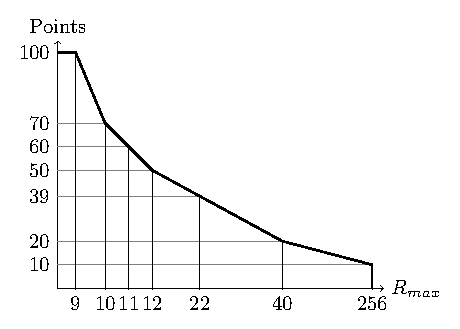
\includegraphics[width=0.7\textwidth]{scoring-en.pdf}

  \parbox{0.4\textwidth}{\centering
    The number of points you get for a given $R_{\max}$.\\
    Note that the x-axis is not linear.
  }
\end{figure}

If $R_{\max} \leq 9$, you get 100 points.
The score values for $9 \leq R_{\max} \leq 20$ are also given in the table below.

\begin{center}
\begin{tabular}{|c|c|c|c|c|c|c|c|c|c|c|c|c|}
  \hline
  $R_{\text{max}}$ & 9 & 10 & 11 & 12 & 13 & 14 & 15 & 16 & 17 & 18 & 19 & 20 \\ \hline
  Points & 100 & 70 & 60 & 50 & 48 & 47 & 46 & 45 & 44 & 43 & 42 & 41 \\ \hline
\end{tabular}
\end{center}

\section*{Sample Judge}
To make it easier to test your program, a sample judge is provided in the attachments at the bottom.
This is not the same judge code that is used on Kattis.
A description of how to run the code is given in the comment at the beginning of the code.

\section*{Explanation of Sample}

\textbf{Note}: the following sample case will not be run against your submission since $N \neq 512$.
It exists only to demonstrate the input and output format; all input that your solution is tested on has $N = 512$.

Initially, all mushrooms have the value $0$.
Below, the mushrooms' values before and after each operation are shown.

\begin{center}
  \noindent
  \begin{tabular}{|c|}
    \hline
    0 0 0 0\\ \hline
    0 1 0 1\\ \hline
    0 1 2 2\\ \hline
  \end{tabular}
\end{center}
